\documentclass[fleqn,compress,utf8,aspectratio=169,t]{beamer}
% use LMU theme
\usetheme{LMU}

% Configuration of listings and common packages
\usepackage{hyperref}
\usepackage{datetime}
\usepackage{verbatim}
\usepackage{longtable,booktabs,tabularx, multirow}
\usepackage[labelformat=empty]{caption}
\usepackage{adjustbox}

\usepackage{listings}

% setup listings
\lstset{
    basicstyle=\ttfamily\color{black},
    showstringspaces=false
}

\lstdefinestyle{highlight}{
    keywordstyle=\color{red},
    commentstyle=\color{lmu@darkgray}
}

\lstdefinestyle{basetex}{
    language={[LaTeX]Tex},
    basicstyle=\color{black!40},
    keywordstyle=\color{red!40},
    commentstyle=\color{lmu@darkgray!40},
    moredelim=**[il][\only<+>{\color{black}\lstset{style=highlight}}]{@}
}

\lstdefinestyle{basec}{
    language=C,
    basicstyle=\color{black!40},
    keywordstyle=\color{red!40},
    commentstyle=\color{green!40},
    moredelim=**[il][\only<+>{\color{black}\lstset{style=highlight}}]{@}
}


\usepackage{physics}
\usepackage{wrapfig}

%%%%%%%%%%%%%%%%%%%%%%%%%%%%%%%%%%%%%%%%%%%%%%%%%%%%%%%%%%%%%%%%%%%%%%%%%%%%%%%%
%%                                  Title Page Data                           %%
%%%%%%%%%%%%%%%%%%%%%%%%%%%%%%%%%%%%%%%%%%%%%%%%%%%%%%%%%%%%%%%%%%%%%%%%%%%%%%%%

% helper command to add multiple authors
\newcommand{\newauthor}[2]{
  \parbox[c]{0.26\textwidth}{
        {\bfseries #1} \\
        {\scriptsize{\href{mailto:#2}{#2}}}
      }
      %{#1}
  }

% Authors
\author[Adrian Uffmann]{
    \newauthor{Adrian Uffmann\inst{1}}{adrian.uffmann@campus.lmu.de}
}

\institute{
    {LMU München}
}

\date[\today]{\today}

\title{Video-Hausarbeit}
\subtitle{Einführung in Quantencomputing}

%%%%%%%%%%%%%%%%%%%%%%%%%%%%%%%%%%%%%%%%%%%%%%%%%%%%%%%%%%%%%%%%%%%%%%%%%%%%%%%%
%%                                  Document                                  %%
%%%%%%%%%%%%%%%%%%%%%%%%%%%%%%%%%%%%%%%%%%%%%%%%%%%%%%%%%%%%%%%%%%%%%%%%%%%%%%%%

\begin{document}

\begin{frame}
 \titlepage
\end{frame}

%%%%%%%%%%%%%%%%%%%%%%%%%%%%%%%%%%% Overview %%%%%%%%%%%%%%%%%%%%%%%%%%%%%%%%%%%

\section{Aufgabe 1a}

\begin{frame}{}
Beispiel für solch einen Zustand in der Basis $\{\ket{+}, \ket{-}\}$ (Hadamard Basis).
\[
\begin{aligned}
\ket{\Psi} &= \hat{\alpha} \cdot \ket{+} + \hat{\beta} \cdot \ket{-} \\
\hat{\alpha}^2 &= 20\% = 0,2
\Rightarrow \hat{\alpha} 
= \sqrt{0,2} 
= \frac{1}{\sqrt5} \\
|\hat{\beta}|^2 &= 1 - |\hat{\alpha}|^2
\Rightarrow |\hat{\beta}| = \pm\sqrt{1 - |\hat{\alpha}|^2}
= \pm\sqrt{1 - |\frac{1}{\sqrt5}|^2}
= \pm\sqrt{1 - \frac{1}{5}}
= \pm\frac{2}{\sqrt5}
\end{aligned}
\]
$\Rightarrow$ Ein Beispiel für $\hat{\beta}$ ist $\frac{2}{\sqrt5}$\\
$\Rightarrow$ Ein Beispiel für $\Psi$ ist $\frac{1}{\sqrt5} \ket{+} + \frac{2}{\sqrt5} \ket{-}$\\
\end{frame}

\begin{frame}{}
Für $\ket{\Phi} = \frac{1}{\sqrt5} \ket{+} + \frac{2}{\sqrt5} \ket{-}$:
\[
\begin{aligned}
H \ket{\Phi}
&= \frac{1}{\sqrt2}
\begin{pmatrix}
1 & 1 \\
1 & -1 \\
\end{pmatrix}
\cdot
\begin{pmatrix}
\frac{1}{\sqrt{5}} \\
\frac{2}{\sqrt{5}} \\
\end{pmatrix}
=
\begin{pmatrix}
\frac{1}{\sqrt{2}} \cdot \frac{1}{\sqrt{5}} + \frac{1}{\sqrt{2}} \cdot \frac{2}{\sqrt{5}} \\
\frac{1}{\sqrt{2}} \cdot \frac{1}{\sqrt{5}} - \frac{1}{\sqrt{2}} \cdot \frac{2}{\sqrt{5}} \\
\end{pmatrix}
=
\begin{pmatrix}
\frac{3}{\sqrt{10}} \\
-\frac{1}{\sqrt{10}} \\
\end{pmatrix}
\\
&=
\frac{3}{\sqrt{10}} \ket{+} - \frac{1}{\sqrt{10}} \ket{-}
\\
\Rightarrow \ket{\Phi} &= \frac{3}{\sqrt{10}} \ket{0} - \frac{1}{\sqrt{10}} \ket{1}
\end{aligned}
\]
\end{frame}

\section{Aufgabe 1b}

\begin{frame}{Komplexität}
\textit{"Quantencomputer sind einfach schnellere Rechner, die Probleme beliebiger Komplexität
im Handumdrehen lösen."}

Das stimmt nicht.

Quantencomputer können alles berechnen, was normale Computer auch berechnen können, \textbf{aber} sie sind nicht bei jedem Problem schneller.

Für Quantenalgorithmen gibt es eine eigene Komplexitätsklasse.

\end{frame}

\begin{frame}{BQP (\textit{bounded error quantum polynomial time})}
\centering
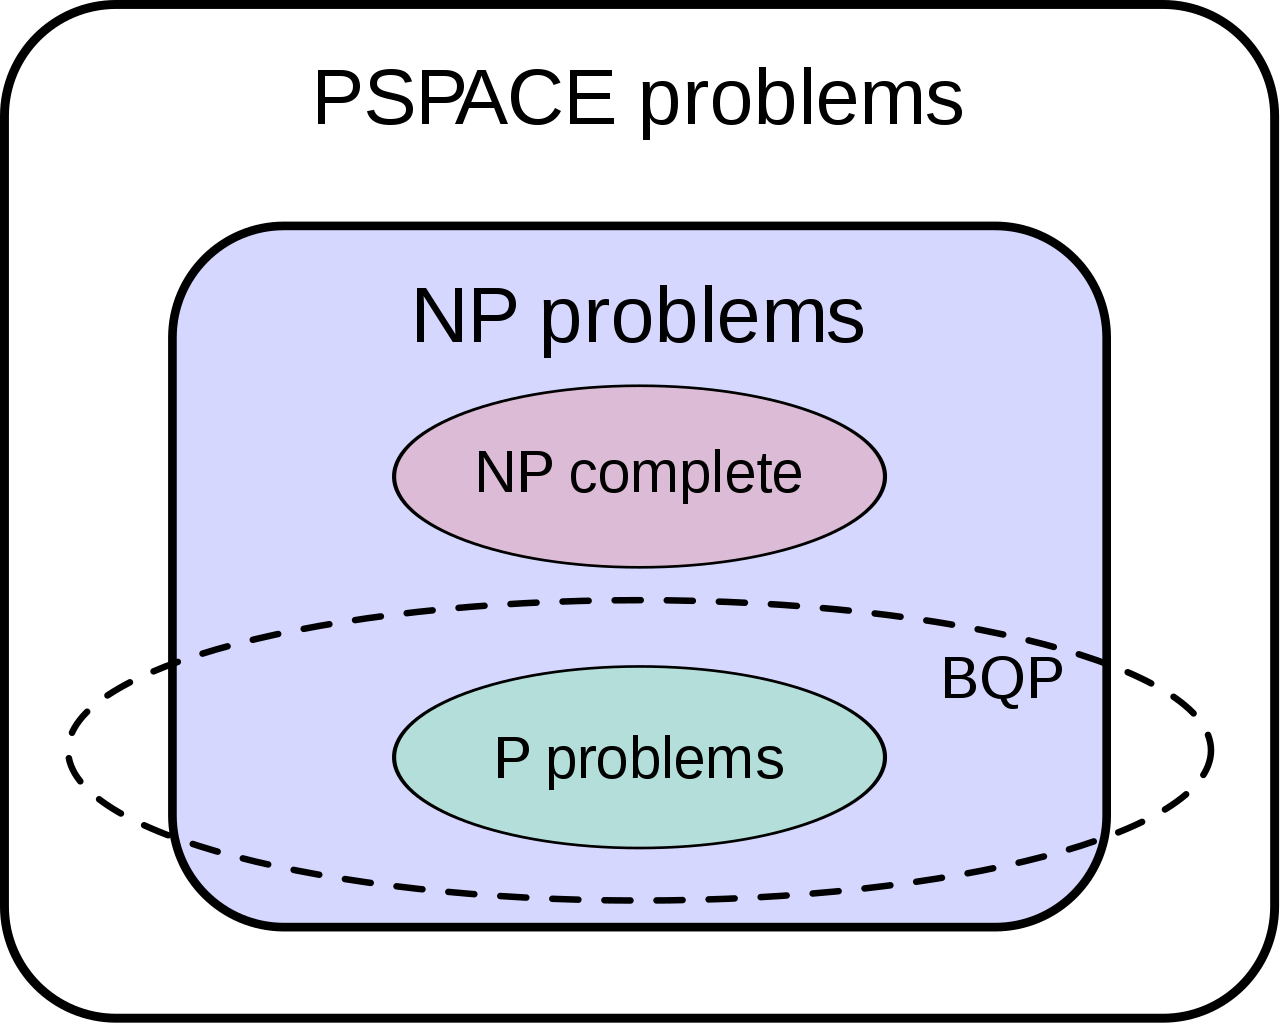
\includegraphics[height=.8\textheight]{images/1280px-BQP_complexity_class_diagram.svg.png}
\end{frame}

\section{Aufgabe 1c}

\begin{frame}{Bell Zustände}
\begin{itemize}
	\item Die Bell-Zustände sind verschränkte Zustände.
	\item lassen sich mit einem sehr einfachen Schaltkreis erzeugen.
\end{itemize}
\begin{figure}
	\centering
	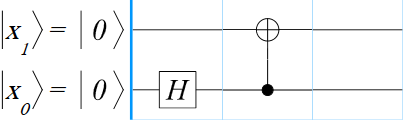
\includegraphics[height=.3\textheight]{images/1c.png}
\end{figure}
\end{frame}

\begin{frame}{Die vier Bell Zustände}
\begin{itemize}
	\item $\ket{\beta_{00}} = \ket{\Phi^+} = \frac{1}{\sqrt{2}} (\ket{00} + \ket{11})$
	\item $\ket{\beta_{10}} = \ket{\Phi^-} = \frac{1}{\sqrt{2}} (\ket{00} - \ket{11})$
	\item $\ket{\beta_{01}} = \ket{\Psi^+} = \frac{1}{\sqrt{2}} (\ket{01} + \ket{10})$
	\item $\ket{\beta_{11}} = \ket{\Psi^-} = \frac{1}{\sqrt{2}} (\ket{01} - \ket{10})$
\end{itemize}
\end{frame}

\section{Aufgabe 1d}

\begin{frame}{SWAP-Gatter logisch}
\begin{itemize}
	\item SWAP-Gatter tauschen die Zustände zweier QuBits.
	\item[$\Rightarrow$] SWAP-Gatter sind logisch gesehen nie nötig, denn man könnte auch mit nicht-vertauschten QUBits weiter rechnen.
\end{itemize}

\begin{figure}
	\begin{minipage}{.5\textwidth}
		\centering
		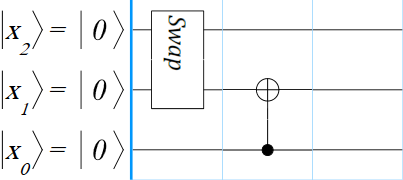
\includegraphics[height=.3\textheight]{images/1d-mit-swap.png}
	\end{minipage}%
	\begin{minipage}{.5\textwidth}
		\centering
		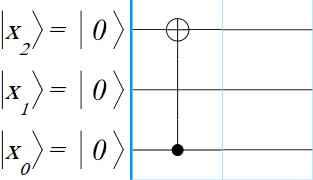
\includegraphics[height=.3\textheight]{images/1d-ohne-swap.png}
	\end{minipage}
\end{figure}
\end{frame}

\begin{frame}{SWAP-Gatter physikalisch}
Echte Quantencomputer ...
\begin{itemize}
	\item ... können kontrollierte Operationen nicht zwischen beliebigen QuBits machen.
	\item ... haben eine Netzwerktopologie.
\end{itemize}
\begin{figure}
	\centering
	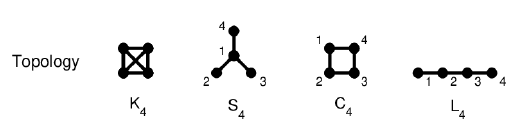
\includegraphics[height=.3\textheight]{images/1d-topologie.png}
	\caption{Beispiel für Netzwerktopologien}
\end{figure}
\end{frame}

\section{Aufgabe 2a}

\begin{frame}{Grover's Algorithmus}
\begin{itemize}
	\item untersucht Funktionen der Form $f: \{0, 1\}^n \rightarrow \{0, 1\}$.
	\item Ziel ist es, eine Eingabe zu finden, bei der die Funktion eine Ausgabe von 1 liefert.
	\item Funktioniert besser, wenn es weniger mögliche Ergebnisse gibt.
	\item Eignet sich für unser Problem, wenn wir eine Funktion finden, die nur für den kürzesten Pfad 1 liefert.
\end{itemize}	
\end{frame}

\begin{frame}{Shor's Algorithmus}
\begin{itemize}
	\item Kann effizient Zahlen faktorisieren.
	\item Eignet sich um RSA zu brechen.
	\item Eignet sich nicht für unser Problem.
\end{itemize}
\end{frame}

\begin{frame}{Quanten Fourier Transformation}
\begin{itemize}
	\item die Quanten-Variante der DFT (\textit{diskrete Fourier-Transformation}).
	\item Eignet sich um die Periode einer Funktion zu finden.
	\item Eignet sich nicht für unser Problem.
\end{itemize}
\end{frame}

\begin{frame}{Simon's Algorithmus}
\begin{itemize}
	\item untersucht Funktionen der Form $f: \{0, 1\}^n \rightarrow \{0, 1\}^n$.
	\item Ziel ist es herauszufinden, ob die Funktion bijektiv ist, oder
	\item ob es einen Vektor $s$ gibt, sodass $f(x) = f(\hat{x}) \Leftrightarrow x \oplus s = \hat{x}$.\\
	($\oplus$ steht hier für element-weises XOR)
	\item Beispiel: Wenn $f(001_2) = f(111_2)$ ist der gesuchte Vektor\\
	$s = 110_2 = 
	\begin{pmatrix}
	0 \\
	1 \\
	1 \\
	\end{pmatrix}$,
	denn $001_2 \oplus 110_2 =
	\begin{pmatrix}
	1 \oplus 0 \\
	0 \oplus 1 \\
	0 \oplus 1 \\
	\end{pmatrix}
	=
	\begin{pmatrix}
	1 \\
	1 \\
	1 \\
	\end{pmatrix}
	= 111_2$
	\item Eignet sich nicht für unser Problem.
\end{itemize}
\end{frame}

\section{Aufgabe 2b}

\begin{frame}{Überlegung: Optimale Funktion}
\begin{itemize}
	\item Mit Grover's Algorithmus erhalten wir für eine Funktion der Form $f: \{0, 1\}^n \rightarrow \{0, 1\}$ eine Eingabe, die eine Ausgabe von 1 erzeugt.
	\item[$\Rightarrow$] Optimal wäre eine Funktion, der man den Pfad als Eingabe gibt und die 1 liefert, genau dann, wenn es der kürzeste Pfad von $S$ zu $Z$ ist.
	\item nur leicht zu implementieren, wenn kürzester Pfad bereits bekannt.
	\item Dazu mehr in Aufgabe 2f.
\end{itemize}
\end{frame}

\begin{frame}{Modellierung der Eingabe}
Die Eingabe muss einen Pfad repräsentieren. Hier gibt es verschiedene Varianten:
\begin{enumerate}
	\item Jedes Bit steht für einen Knoten (gesetzt bedeutet Teil des Pfades).
	\item[] $\Rightarrow$ Pfad nicht eindeutig, Knoten-Reihenfolge nicht klar.
	\item Jedes Bit steht für eine Kante (gesetzt bedeutet Teil des Pfades).
	\item[] $\Rightarrow$ Pfad schwer zu validieren, da Kanten-Reihenfolge implizit.
	\item Mehrere Bits kodieren einen Knoten, mehrere kodierte Knoten ergeben den Pfad.
	\item[] $\Rightarrow$ Leicht zu validieren, da Knote-Reihenfolge Teil der Eingabe.
	\item Mehrere Bits kodieren eine Kante, mehrere kodierte Kanten ergeben den Pfad.
	\item[] $\Rightarrow$ Wie 3., aber es gibt mehr Kanten als Knoten, daher ineffizienter.
\end{enumerate}
\end{frame}

\begin{frame}{Modellierung der Eingabe}
Wir verwenden Variante 3.

Bei vier Knoten $\{a, b, c, d\}$ reichten 2 Bit um einen Knoten zu kodieren:\\
$a = \ket{00}$, $b = \ket{01}$, $c = \ket{10}$ und $d = \ket{11}$.

Wir schreiben Knoten, die weiter vorne im Pfad sind auf die QBits mit niedrigerem Index (also weiter rechts).

Z.~B. wird der Pfad $b \rightarrow c \rightarrow a$ als $\ket{001001}$ dargestellt.
\end{frame}

\begin{frame}{Modellierung von Startknoten und Zielknoten}
\begin{itemize}
	\item Ein valider Pfad muss immer bei $S$ beginnen und bei $Z$ enden.
	\item[$\Rightarrow$] Wir müssen nur den Teilpfad zwischen $S$ und $Z$ betrachten.
	\item Es macht keinen Sinn, wenn $S$ oder $Z$ an anderer Stelle im Pfad auftauchen.
	\item[$\Rightarrow$] Wir brauchen keine Zahlen um $S$ und $Z$ kodieren zu können.
\end{itemize}
\end{frame}

\begin{frame}{Funktionsdefinition}
\begin{itemize}
	\item Der Graph hat nur einen kürzesten Pfad: $S \rightarrow a \rightarrow Z$.
	\item Dieser wird als $\ket{00}$ dargestellt.
	\item[$\Rightarrow$] $f(x) = \begin{cases}
	1 & x = \ket{00}\\
	0 & \text{otherwise.}\\
	\end{cases}$
\end{itemize}
\end{frame}

\section{Aufgabe 2c}

\begin{frame}{}
\begin{figure}
\centering
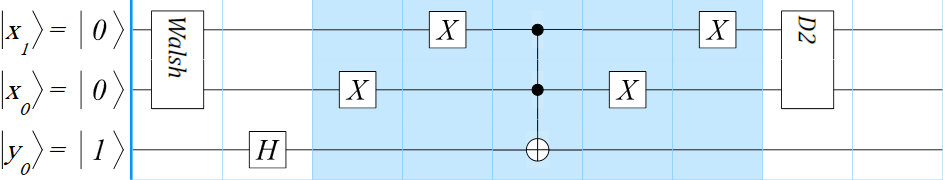
\includegraphics[width=\textwidth]{images/2c.png}
\caption{$U_f$ ist blau hinterlegt}
\end{figure}
Als Erinnerung $f(x) = \begin{cases}
1 & x = \ket{00}\\
0 & \text{otherwise.}\\
\end{cases}$
\end{frame}

\section{Aufgabe 2d}

\begin{frame}{}
\begin{minipage}[t]{.333\textwidth}
\centering
Zustand vor $U_f$:
\begin{figure}
	\includegraphics[width=.9\textwidth]{images/2d-vor-UF.png}
\end{figure}
\end{minipage}%
\begin{minipage}[t]{.333\textwidth}
\centering
Zustand nach $U_f$:
\begin{figure}
	\includegraphics[width=.9\textwidth]{images/2d-nach-UF.png}
\end{figure}
\end{minipage}%
\begin{minipage}[t]{.333\textwidth}
\centering
Ergebniszustand:
\begin{figure}
	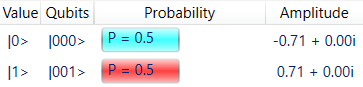
\includegraphics[width=.9\textwidth]{images/2d-nach-D2.png}
\end{figure}
\end{minipage}%
\end{frame}

\section{Aufgabe 2e}

\begin{frame}{Kürzeste Wege}
Es gibt 7 kürzeste Wege (alphabetisch sortiert):
\begin{enumerate}
	\item $S \rightarrow i \rightarrow a \rightarrow d \rightarrow Z$
	\item $S \rightarrow i \rightarrow a \rightarrow e \rightarrow Z$
	\item $S \rightarrow i \rightarrow a \rightarrow g \rightarrow Z$
	\item $S \rightarrow i \rightarrow h \rightarrow d \rightarrow Z$
	\item $S \rightarrow l \rightarrow c \rightarrow d \rightarrow Z$
	\item $S \rightarrow l \rightarrow c \rightarrow j \rightarrow Z$
	\item $S \rightarrow l \rightarrow h \rightarrow d \rightarrow Z$
\end{enumerate}
\end{frame}

\begin{frame}{Abändern der Funktion}
Dieser Graph hat 2 Unterschiede:
\begin{enumerate}
	\item Es gibt mehr Knoten 12 und $S$ und $Z$.
	\item[$\Rightarrow$] Es werden nun $ceil(log_2(12)) = 4$, statt 2 Bits pro Knoten benötigt.
	\item Es gibt mehr kürzeste Pfade.
	\item[$\Rightarrow$] Bei allen muss die Funktion 1 liefern.
\end{enumerate}
\end{frame}

\begin{frame}{Abändern des Schaltkreises}
\begin{minipage}[t]{.65\textwidth}
Eingabedarstellung der zwei ersten kürzesten Pfade:
\begin{enumerate}
	\item $S \rightarrow i \rightarrow a \rightarrow d \rightarrow Z \equiv \ket{001100001000}$
	\item $S \rightarrow i \rightarrow a \rightarrow e \rightarrow Z \equiv \ket{010000001000}$
\end{enumerate}

Die Schaltkreise für die kürzesten Pfade können einfach hintereinander ausgeführt werden.

Aufeinander folgende X-Gatter können weggelassen werden.
\end{minipage}%
\begin{minipage}[t]{.35\textwidth}
\begin{figure}
	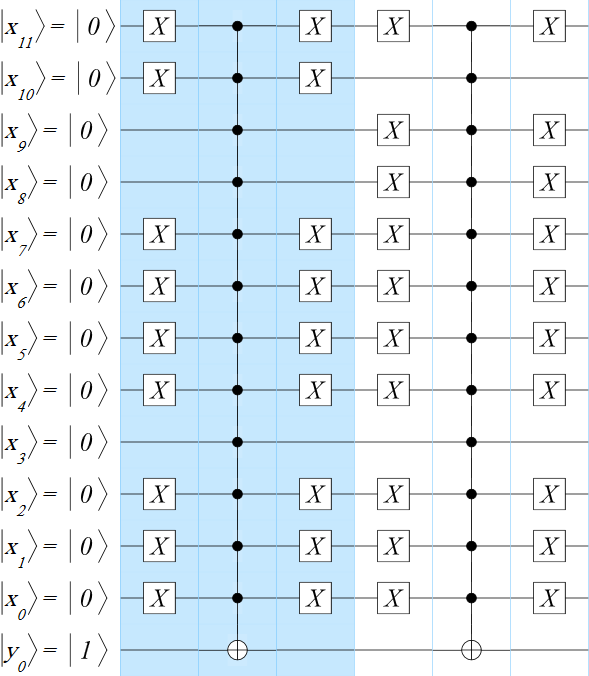
\includegraphics[height=.6\textheight]{images/2e.png}
	\caption{Teile des Orakels: blau für Pfad 1, weiß für Pfad 2.}
\end{figure}
\end{minipage}
\end{frame}

\begin{frame}{Zustand nach $U_f$}

\begin{minipage}[t]{.65\textwidth}
\begin{itemize}
	\item Ähnlich wie in 2d.
	\item Das angepasste Orakel wird bei 7 statt nur einem Pfad aktiv.
	\item[$\Rightarrow$] Es sollten bei 14 statt nur bei 2 Zuständen der Superposition die Vorzeichen negiert worden sein.
\end{itemize}

\end{minipage}%
\begin{minipage}[t]{.35\textwidth}
\begin{figure}
	\includegraphics[width=\textwidth]{images/2d-nach-UF.png}
	\caption{Zustand nach $U_f$ aus Aufgabe 2d}
\end{figure}
\end{minipage}
\end{frame}

\section{Aufgabe 2f}

\begin{frame}{Verallgemeinerung des Schaltkreises}
\begin{itemize}
	\item Bisherige Annahme: Funktion liefert 1, genau dann, wenn Eingabe der kürzeste Pfad von $S$ zu $Z$.
	\item \textbf{Aber:} Im Allgemeinen zu schwer, man kann nicht leicht prüfen, ob kürzerer Pfad existiert.
	\item Wie beim Max-Cut-Problem reicht es, wenn die Funktion nur für valide Pfade mit bestimmter Länge eine 1 liefert.
	\item[$\Rightarrow$] Dann kann mit binärer Suche die kürzeste Länge bestimmt werden.
\end{itemize}
\end{frame}

\begin{frame}{Abbilden des Problems in eine analysierbare Funktion}
\begin{itemize}
	\item Unsere Funktion soll nur für valide Pfade mit bestimmter Länge eine 1 liefern.
	\item Die Pfadlänge ist durch die Länge der Eingabe bereits festgelegt.
	\item[$\Rightarrow$] Die Funktion muss daher nur noch den Pfad validieren.
\end{itemize}
\end{frame}

\begin{frame}{Welche Eigenschaften hat ein valider Pfad?}
\begin{enumerate}
	\item Der erste Pfad-Knoten muss durch eine Kante mit $S$ verbunden sein.
	\item Für aufeinander folgende Knoten muss der Graph eine Kante enthalten.
	\item Der letzte Pfad-Knoten muss durch eine Kante mit $Z$ verbunden sein.
\end{enumerate}
\begin{itemize}
	\item Die Eigenschaften lassen sich leicht prüfen, indem für jedes aufeinander folgende Knotenpaar geprüft wird, ob es so eine Kante gibt.
	\item Wenn ja wird der Wert in einem Ancilla QuBit gespeichert.
	\item Die Ancilla QBits können dann mit einem mehrfachen Toffoli verundet werden.
	\item[$\Rightarrow$] Es werden so viele Ancilla QuBits benötigt, wie der Pfad Kanten hat.
\end{itemize}

\end{frame}

\begin{frame}{Allgemeines Orakel für Problem aus 2b}
\begin{minipage}{.75\textwidth}
	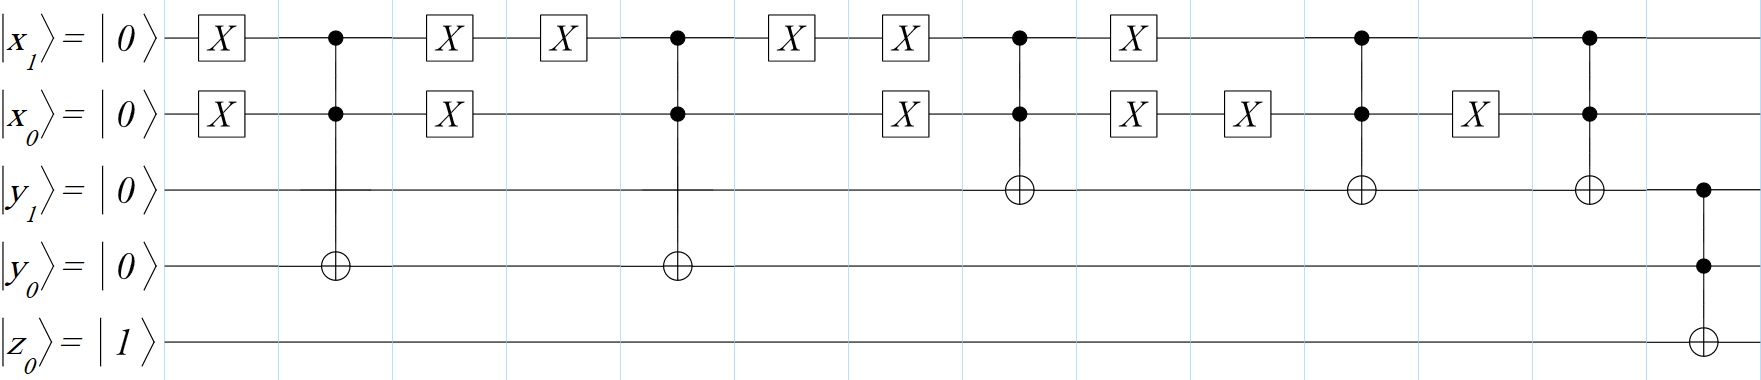
\includegraphics[width=.95\textwidth]{images/2f.png}
\end{minipage}%
\begin{minipage}{.25\textwidth}
	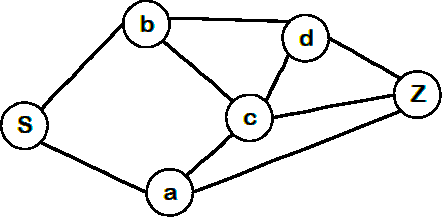
\includegraphics[width=.95\textwidth]{images/2-graph.png}
\end{minipage}
\begin{itemize}
	\item $y_0$: gibt es eine Kante zwischen $S$ und dem ersten (einzigen) Knoten des Pfades.
	\item $y_1$: gibt es eine Kante zwischen dem letzten (einzigen) Knoten des Pfades und $Z$.
	\item Anschließend werden die Ancilla QuBits wieder entschränkt, indem die Operationen (außer das letzte Toffoli) noch einmal rückwärts ausgeführt werden.
\end{itemize}
\end{frame}

\section{Aufgabe 2g}

\begin{frame}{Laufzeit}

Die Laufzeit hängt von der Anzahl der Knoten $V$, der Anzahl der Kanten $E$ und der Länge des zu untersuchenden Pfades $|P|$ ab.

Das Orakel aus 2f benötigt für jede Kante des Pfades eine zu der Anzahl der Knoten logarithmische Anzahl an Operationen pro Kante des Graphes. Das Orakel hat also eine Komplexität von $O(|P| \cdot |E| \cdot log(|V|))$.

Dies muss man noch multiplizieren mit der Anzahl der Aufrufe des Orakels.

Diese hängt logarithmisch von der Größe des Suchraumes der binären Suche und von der optimalen Anzahl von Grover-Iterationen ab.
\end{frame}

\begin{frame}{Laufzeit}

Die binäre Suche liegt in $O(log(|V|))$, da der kürzeste Pfad höchstens alle Knoten besucht.

Das Register $x$, auf dem Grover's Algorithmus agiert hat eine Größe $n$ in $O(|P| \cdot log(|V|))$, da $O(|P|)$ Knoten in der Eingabe sind und jeder $O(log(|V|))$ QuBits für die Kodierung braucht.

Die optimale Anzahl an Grover-Iterationen bei $M$ mögichen Messergebnissen liegt in $O(\sqrt{\frac{2^{n}}{M}})$.

Es ist also nicht offensichtlich, ob der Algorithmus den klassischen Algorithmus von Dijkstra mit $O(|E| + |V| log(|V|))$ schlagen kann.
\end{frame}

\section{Aufgabe 3a}

\begin{frame}{Dekohärenz}
\begin{itemize}
	\item ist das Phänomen, dass QuBits mit der Umgebung interagieren können.
\end{itemize}

Beispiel aus der Vorlesung:

\begin{minipage}{.5\textwidth}
\centering
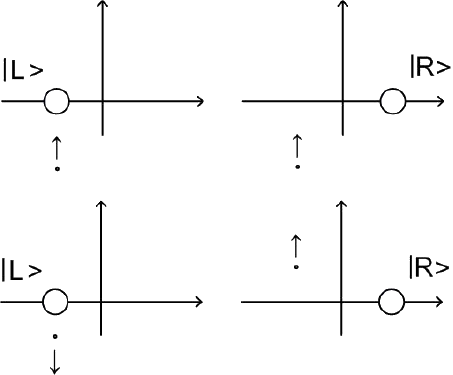
\includegraphics[width=.7\textwidth]{images/3a.png}
\end{minipage}%
\begin{minipage}{.5\textwidth}
\centering
$\frac{1}{\sqrt2}(\ket{L} + \ket{R}) \ket{\uparrow} = \frac{1}{\sqrt2}(\ket{L} \ket{\uparrow} + \ket{R} \ket{\uparrow})$

\vspace{1em}

$\xrightarrow{\text{Interaktion}}$

\vspace{1em}

$\frac{1}{\sqrt2}(\ket{L} \ket{\downarrow} + \ket{R} \ket{\uparrow})$
\end{minipage}%
\end{frame}

\begin{frame}{Dekohärenz Vermeidung}
Um Dekohärenz zu vermeiden werden Quantencomputer stark gekühlt und von äußeren Einflüssen isoliert.
\end{frame}

\section{Aufgabe 3b}

\begin{frame}{Warum ist Fehlerkorrektur in Quantencomputern schwieriger?}
\begin{itemize}
	\item No-Cloning Theorem.
	\item In einem diskreten System können sich Fehler leichter aufaddieren.
\end{itemize}
\end{frame}

\section{Aufgabe 3c}

\begin{frame}{\textit{Bitflip} vs. \textit{Phaseflip}}
\begin{itemize}
	\item \textit{Bitflip}
	\begin{itemize}
		\item kennt man auch aus der klassischen Informatik.
		\item an einer Stelle, an der eine 0 sein sollte, ist eine 1 (oder anders herum).
		\item entspricht der Anwendung eines X-Gatters.
	\end{itemize}
	\item \textit{Phaseflip}
	\begin{itemize}
		\item Die Amplitude von $\ket{1}$ hat das falsche Vorzeichen (Minus statt Plus, oder anders herum).
		\item entspricht der Anwendung eines Z-Gatters.
	\end{itemize}
\end{itemize}
Da sowohl das X-Gatter, als auch das Z-Gatter ihre eigenen Inversen sind, können diese Gatter die Fehler auch wieder beheben.
\end{frame}

\section{Aufgabe 3d}

\begin{frame}{Dichte Kodierung}
\end{frame}

\end{document}
